\chapter{Memory Efficient Incremental LOF with RKNN}\label{Memory Efficient Incremental LOF with RKNN}

\section{Introduction}


Outlier detection techniques of static data does not help to solve real time problems because we have to deal with streaming data. Outlier detection on streaming data is particularly
challenging, since the volume of data to be analyzed is
effectively unbounded and cannot be stored indefinitely in
memory for processing. Hence some of the data points are selected and clustered so that each of the cluster centers can represent the selected data points. These data points are further deleted to free up memory. The selection of points which are to be deleted is crucial because these points may affect the computation of LOF of upcoming data points. In MiLOF, points which come earlier are deleted whenever memory limit is reached.  


\section{Related Work}

%Local Outlier Factor is a score for each of the data points that represents the degree of anomalous behavior for that point. For the point deep inside a cluster it is nearly equal to 1. We first compute the K-distances by finding K nearest neighbors of the points. After computing K-siatances, lrd and LOF value is computed.
%\par

LOF score is the criteria to know if a data point is outlier or not. To compute LOF of data points in data streams, incremental LOF technique is used. In incremental LOF(iLOF), LOF is computed for each of the data points from the data stream. But the assumption there is that memory available is infinity. 

\par
Storing all the data points in data stream is impractical because that need a huge memory space. Moreover the time complexity to measure LOF will be increasing if the size is increasing. So to implement incremental LOF with limited memory , Memory efficient Incremental LOF (MiLOF) was developed. 

\par If total available memory is just sufficient to store $K$-distance, lrd and LOF of $m$ data points then this memory is divided into two parts of size $b$ and $c$ to store $b$ original data points and $c$ summarized cluster centers respectively. For every new incoming data point LOF in computed following iLOF using the information of b$ $original data points and $c$ cluster centers. If memory limit is reached, first half of the data points are removed from the memory. They are summarized into $c$ clusters and then merged with the previous cluster centers using weighted $K$-means algorithm. Weight here for a cluster center is number of data points in that cluster. This way incremental LOF computation in data stream is done in memory efficient way.






 \section{Proposed Work}
 In MiLOF what we are doing is that we are selecting the points which came first. But this selection of points can cost us accuracy for computation of LOF  upcoming points. Hence selection of points which are to be summarized is very crucial. In MiLOF whenever the number of data points in memory reaches $b$, half of the points are selected to be summarized and deleted. But on what basis we should select these points to increase accuracy. In MiLOF, they choose the first $\frac{b}{2}$ points on their arrival time basis. There must be some other parameter that can help to decide which points to be deleted.

To deal with this problem, we propose MiLOF with reverse $K$ nearest neighbor(RKNN) that precisely tells us which points are to be removed. Along with $K$-distance, lrd, LOF of all the points, we store no of reverse KNN for each of these points. \\

\par 
\textbf{Reverse $K$ Nearest Neighbors RKNN(p) } : It is the no of data points which include $p$ in their respective $K$ nearest neighbors.\\

Having stored RKNN for all the $b$ data points, we sort these $b$ points according to RKNN and select $\frac{b}{2}$ data points with highest RKNN. These points are definitely normal points because they have enough neighbors. Hence by removing these points we are keeping candidate outliers for further computation. It can be seen from the results in next section that this reduces false alarm significantly.
Memory distribution is shown in Figure 3.1.


\begin{figure}[H]
	\centering
	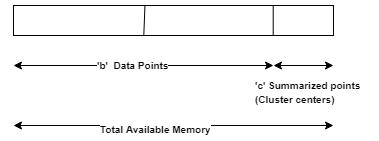
\includegraphics{chap04/partition.png}
	\caption{2-D Dataset used for LOF}
\end{figure}




Algorithm 6 explains MiLOF with RKNN. 

\begin{algorithm}[H]
	\caption{MiLOF with RKNN}
	\begin{algorithmic}
		\STATE  
		\STATE INPUT:  A data point p 
		\STATE OUTPUT: LOF value LOF(p)
		\STATE
		
		\STATE Compute LOF of p and update RKNN for all the data points 
		\IF {No of points=b}
		
		\STATE Sort these b data points according to their RKNN count in decreasing order
		
		\STATE $C^i$ $\leftarrow$ First $\frac{b}{2}$ points
		\STATE ($V^i$,$N^i$) $\leftarrow$ C-means($C^i$)
		
		\FOR {all $v^i$ \in $V^i$} 
		\STATE Compute avereage K-distance, lrd and LOF
		\ENDFOR
		
		\STATE Delete $C^i$
		
		\IF{i>0}
		\STATE (Z;W) $\leftarrow$ Weighted c-means($V^i$ U $V^{i-1}$ ,$N^i$ U $N^{i-1}$)
		
		\FOR {all z \in Z} 
		\STATE Compute avereage K-distance, lrd and LOF
		\ENDFOR 
		\STATE $V^{i-1}$ \leftarrow Z
		\STATE Delete $V^{i-1}$,Z
		
		\ENDIF	
		\ENDIF
		
		\STATE i $\leftarrow$ i+1
		\RETURN LOF
	\end{algorithmic}
\end{algorithm}



\section{Experimental Results}
We computed different performance measures for both the algorithm MiLOF and MiLOF with RKNN and compared their results.
 First of all we computed LOF values for each of the data points taking all of them together. After computing LOF values we classified all the points and recorded the outliers. We used these data points as data stream and computed LOF values using MiLOF and MiLOF with RKNN.  

\subsection{LOF}
Implementation of LOF on a 
a synthetic 2-D dataset with 3 clusters of varying density. 
Dataset description\\
\begin{table}[H]
	\centering
	\caption{2-D Synthetic Dataset description}
	\label{my-label}
	\begin{tabular}{|l|l|}
		\hline
		& \multicolumn{1}{c|}{2-D synthetic dataset} \\ \hline
		\multicolumn{1}{|c|}{$n$: Data points} & \multicolumn{1}{c|}{1500}                  \\ \hline
		
		\multicolumn{1}{|c|}{$d$: Dimensions}  & \multicolumn{1}{c|}{2}                     \\ \hline
		\multicolumn{1}{|c|}{$c$: Clusters}  & \multicolumn{1}{c|}{3}                     \\ \hline
		
		
		
		Noise Points                         & \multicolumn{1}{c|}{50}                                         \\ \hline
	\end{tabular}
\end{table}

\begin{figure}[H]
	\centering
	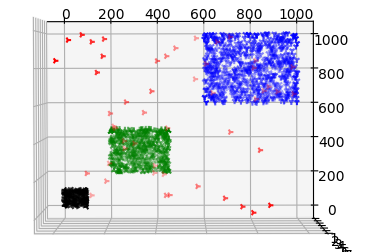
\includegraphics{chap04/LOF_dataset.png}
	\caption{2-D Dataset used for LOF}
\end{figure}

It can be seen from Figure 3.3 that points inside a cluster has LOF values nearly equal to 1 where as noisy points have LOF up to 7. More the LOF score more is the degree of anomaly.

\begin{figure}[H]
	\centering
	\includegraphics{chap04/LOF_result.png}
	\caption{LOF values for synthetic 2-D dataset}
\end{figure}


\subsection{MiLOF and MiLOF with RKNN}

We have implemented MiLOF and MiLOF with RKNN in two datasets and measured their efficiency.

\subsubsection{Performance measures}
Simple accuracy and precision is not the correct measure for these unsupervised anomaly detection problems because the two classes, normal and anomalous are not distributed evenly. So to compare their performance, we compare their false positive rate FPR versus true positive rate TPR.

These performance measures are listed below


\[  Precision \, P = \frac{True Positive }{True Positive + False Positive} \]

\[  Recall \,  R = \frac{True Positive }{True Positive + False Negative} \]

\[  Flase \, Positive \, Rate \,  (FPR) = \frac{False Positive }{False Positive + True Negative} \]
\\
\\


\begin{itemize}
	
	\item \textit{True Positive} : Outliers  predicted as outlier
	 
	\item \textit{True Negative} : Normal points predicted as normal points
	
	\item \textit{False Positive} : Normal points predicted as outliers
	
	
	\item \textit{False Negative } : Outliers  predicted as normal points
	
	
	
	
\end{itemize}

\subsubsection{Dataset}
\begin{table}[H]
	\centering
	\caption{Dataset Description}
	\label{my-label}
	\begin{tabular}{|c|c|l|}
		\hline
		\multicolumn{1}{|l|}{} & UCI Letter Dataset & UCI PenDigit Dataset \\ \hline
		$n$: Data points         & 20000              & 10000                \\ \hline
		$d$: Dimensions          & 16                 & 16                   \\ \hline
		$c$: Classes             & 26                 & 10                   \\ \hline
	\end{tabular}
\end{table}



\subsubsection{UCI Letter Dataset}

Following are the reults of different performance measure parameters for both the algorithm by varying $K$ and $b$(available memory) in UCI letter dataset. 



\begin{table}[H]
	\centering
	\caption{MiLOF and MiLOF with RKNN when $K$ changes while $b$ is kept constant}
	
	\label{my-label}
	\begin{tabular}{|c|c|c|c|c|c|c|c|c|}
		\hline
		\multicolumn{1}{|l|}{}    & \multicolumn{4}{c|}{MiLOF}                                                                                                    & \multicolumn{4}{c|}{MiLOF with RKNN}                                                                                          \\ \hline
		\multicolumn{1}{|l|}{$K$}   & \multicolumn{1}{l|}{Precision} & \multicolumn{1}{l|}{TPR} & \multicolumn{1}{l|}{FPR} & \multicolumn{1}{l|}{TPR/FPR} & \multicolumn{1}{l|}{Precision} & \multicolumn{1}{l|}{TPR} & \multicolumn{1}{l|}{FPR} & \multicolumn{1}{l|}{TPR/FPR} \\ \hline
		\multicolumn{1}{|l|}{100} & 0.132                          & 0.821                              & 0.1154                   & 7.11                         & 0.348                          & 0.727                              & 0.073                    & 9.945                        \\ \hline
		200                       & 0.12                           & 0.874                              & .146                     & 5.96                         & 0.183                          & 0.704                              & 0.076                    & 9.8                          \\ \hline
		300                       & 0.139                          & 0.84                               & 0.1546                   & 5.441                        & 0.255                          & 0.772                              & 0.069                    & 11.561                       \\ \hline
		400                       & 0.184                          & 0.828                              & 0.140                    & 5.88                         & 0.272                          & 0.804                              & 0.821                    & 9.77                         \\ \hline
		500                       & 0.195                          & 0.781                              & 0.157                    & 4.99                         & 0.305                          & 0.761                              & 0.766                    & 9.70                         \\ \hline
		600                       & 0.229                          & 0.772                              & 0.134                    & 5.536                        & 0.355                          & 0.74                               & 0.072                    & 10.252                       \\ \hline
		700                       & 0.221                          & 0.708                              & 0.141                    & 5.01                         & 0.332                          & 0.591                              & 0.067                    & 8.746                        \\ \hline
	\end{tabular}
\end{table}

\begin{figure}[H]
	\centering
	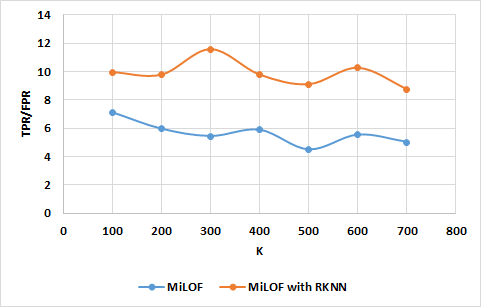
\includegraphics{chap04/varyK.png}
	\caption{TPR/FPR for MiLOF and MiLOF with RKNN when $K$ changes while $b$ is kept constant }
\end{figure}

\begin{table}[H]
	\centering
	\caption{MiLOF and MiLOF with RKNN when $b$ changes while $K$ is kept constant}
	\label{my-label}
	\begin{tabular}{|l|c|c|c|c|c|c|c|c|}
		\hline
		& \multicolumn{4}{c|}{MiLOF}                                                                                                    & \multicolumn{4}{c|}{MiLOF with RKNN}                                                                                          \\ \hline
		$b$                          & \multicolumn{1}{l|}{Precision} & \multicolumn{1}{l|}{TPR} & \multicolumn{1}{l|}{FPR} & \multicolumn{1}{l|}{TPR/FPR} & \multicolumn{1}{l|}{Precision} & \multicolumn{1}{l|}{TPR} & \multicolumn{1}{l|}{FPR} & \multicolumn{1}{l|}{TPR/FPR} \\ \hline
		2000                       & 0.222                          & 0.707                              & 0.141                    & 5.018                        & 0.332                          & 0.59                               & 0.08                     & 7.35                         \\ \hline
		\multicolumn{1}{|c|}{4000} & 0.291                          & 0.908                              & 0.126                    & 7.215                        & 0.467                          & 0.839                              & 0.054                    & 15.443                       \\ \hline
		\multicolumn{1}{|c|}{5000} & 0.308                          & 0.814                              & 0.103                    & 7.83                         & 0.515                          & 0.856                              & 0.045                    & 18.725                       \\ \hline
		\multicolumn{1}{|c|}{8000} & 0.36                           & 0.915                              & 0.092                    & 9.927                        & 0.67                           & 0.883                              & 0.022                    & 40.89                        \\ \hline
	\end{tabular}
\end{table}


\begin{figure}[H]
	\centering
	\includegraphics{chap04/varyb.png}
	\caption{TPR/FPR for MiLOF and MiLOF with RKNN when $b$ changes while $K$ is constant}
\end{figure}

\subsubsection{UCI Pendigit Dataset}

Following are the reults of different performance measure parameters for both the algorithm by varying K and b(available memory) in UCI pendigit dataset. 

\begin{table}[H]
	\centering
	\caption{MiLOF and MiLOF with RKNN when $K$ changes while $b$ is kept constant}
	\label{my-label}
	\begin{tabular}{|l|c|c|c|c|c|c|c|c|}
		\hline
		& \multicolumn{4}{c|}{MiLOF}                                                                                                    & \multicolumn{4}{c|}{MiLOF with RKNN}                                                                                          \\ \hline
		K                         & \multicolumn{1}{l|}{Precision} & \multicolumn{1}{l|}{TPR} & \multicolumn{1}{l|}{FPR} & \multicolumn{1}{l|}{TPR/FPR} & \multicolumn{1}{l|}{Precision} & \multicolumn{1}{l|}{TPR} & \multicolumn{1}{l|}{FPR} & \multicolumn{1}{l|}{TPR/FPR} \\ \hline
		100                       & 0.618                          & 0.823                              & 0.05                     & 10.98                        & 0.786                          & 0.432                              & 0.0173                   & 24.927                       \\ \hline
		\multicolumn{1}{|c|}{200} & 0.59                           & 0.844                              & 0.099                    & 8.48                         & 0.85                           & 0.463                              & 0.1379                   & 33.569                       \\ \hline
		\multicolumn{1}{|c|}{300} & 0.59                           & 0.783                              & 0.084                    & 9.23                         & 0.773                          & 0.53                               & 0.024                    & 21.748                       \\ \hline
		\multicolumn{1}{|c|}{400} & 0.584                          & 0.7723                             & 0.081                    & 9.455                        & 0.789                          & 0.541                              & 0.0214                   & 25.212                       \\ \hline
		500                       & 0.6203                         & 0.688                              & 0.059                    & 11.628                       & 0.851                          & 0.46                               & 0.011                    & 40.48                        \\ \hline
		600                       & 0.651                          & 0.719                              & 0.045                    & 15.97                        & 0.84                           & 0.67                               & 0.015                    & 44.45                        \\ \hline
		700                       & 0.534                          & 0.739                              & 0.059                    & 12.486                       & 0.797                          & 0.508                              & 0.112                    & 43.65                        \\ \hline
	\end{tabular}
\end{table}



\begin{figure}[H]
	\centering
	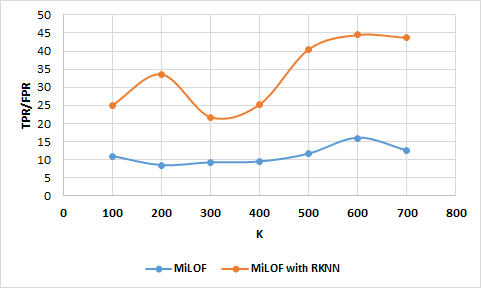
\includegraphics{chap04/varyK2.png}
	\caption{TPR/FPR for MiLOF and MiLOF with RKNN when $K$ changes while $b$ is constant}
\end{figure}



\begin{table}[H]
	\centering
	\caption{MiLOF and MiLOF with RKNN when $b$ changes while $K$ is kept constant}
	\label{my-label}
	\begin{tabular}{|l|c|c|c|c|c|c|c|c|}
		\hline
		& \multicolumn{4}{c|}{MiLOF}                                                                                                    & \multicolumn{4}{c|}{MiLOF with RKNN}                                                                                          \\ \hline
		b                          & \multicolumn{1}{l|}{Precision} & \multicolumn{1}{l|}{TPR} & \multicolumn{1}{l|}{FPR} & \multicolumn{1}{l|}{TPR/FPR} & \multicolumn{1}{l|}{Precision} & \multicolumn{1}{l|}{TPR} & \multicolumn{1}{l|}{FPR} & \multicolumn{1}{l|}{TPR/FPR} \\ \hline
		1000                       & 0.218                          & 0.360                              & .119                     & 3.035                        & 0.1366                         & 0.2158                             & 0.126                    & 1.72                         \\ \hline
		\multicolumn{1}{|c|}{2000} & 0.462                          & 0.412                              & 0.044                    & 9.33                         & 0.471                          & 0.281                              & 0.029                    & 9.678                        \\ \hline
		\multicolumn{1}{|c|}{4000} & 0.5723                         & 0.750                              & 0.052                    & 14.54                        & 0.78                           & 0.65                               & 0.017                    & 38.33                        \\ \hline
		\multicolumn{1}{|c|}{5000} & 0.590                          & 0.794                              & 0.05                     & 15.6                         & 0.79                           & 0.878                              & 0.021                    & 41.22                        \\ \hline
	\end{tabular}
\end{table}

\begin{figure}[H]
	\centering
	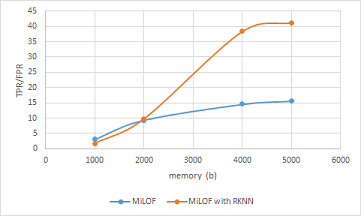
\includegraphics{chap04/varyB2.png}
	\caption{TPR/FPR for MiLOF and MiLOF with RKNN when $K$ changes while $b$ is constant}
\end{figure}



\section{Conclusion}

In MiLOF with RKNN we are selecting the points which have high RKNN counts to be deleted. High RKNN count means that the point is surrounded by many data points. These points are most likely to be normal points. Clustering these points and deleting is safer than deleting points with low RKNN count because they are candidate outliers. There is an ambiguity for the points with low RKNN values whether they are outlier or not. But points with high RKNN values are definitely not outliers. Hence these points are deleted. From the results it is clear that MiLOF with RKNN has significantly low False Positive Rate than MiLOF.






